\chapter{序論}
\section{背景}
近年,様々なセンサを用いた自律走行に関する研究が盛んに行われており,
その中でカメラ画像を用いてロボットへ自律走行を行わせる研究も行われている.
%\index{うえだ@上田}
%例として,\cite{上田2015gihyo,ueda2015,上田2015jsai}がある.
Bojaskiら\cite{Nvidia}は
Fig. \ref{fig::nvidia}で示す方法で,人間のハンドル操作によるステアリングの角度の模倣学習を行い,
画像を用いて走行を行う方法を提案した.

\begin{figure}[h]
    \centering
    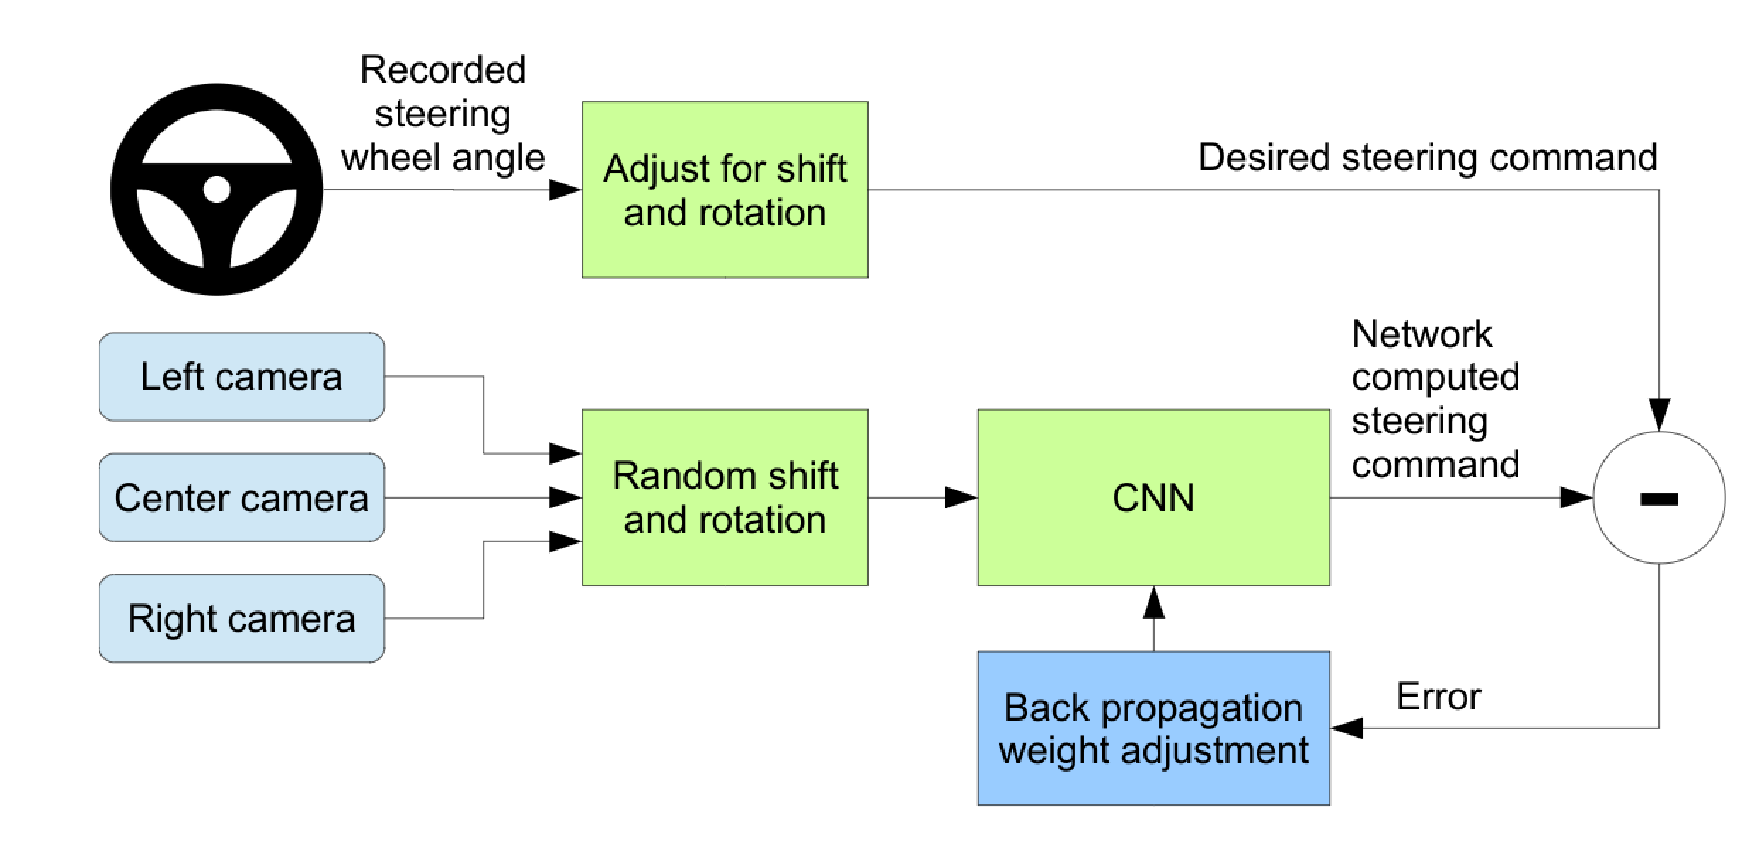
\includegraphics[width = 13cm]{./figs/EndtoEnd_Learning_for_Self-Driving_Cars.pdf}
    \caption{Training the neural network from \cite{Nvidia}}
    \label{fig::nvidia}
\end{figure}

\newpage
本研究室においても岡田ら\cite{okada}はFig. \ref{fig::okada}に示すような経路追従行動を,
行動を模倣し,カメラ画像を用いた経路追従行動を獲得した.
研究ではFig. \ref{fig::okada_sys}に示すように,
LiDAR,オドメトリの入力としたルールベース制御器(後述する"地図べースの制御器")による経路追従行動を行い,
その行動をカメラ画像を用いてend-to-endで模倣学習している.
\begin{figure}[h]
    \centering
    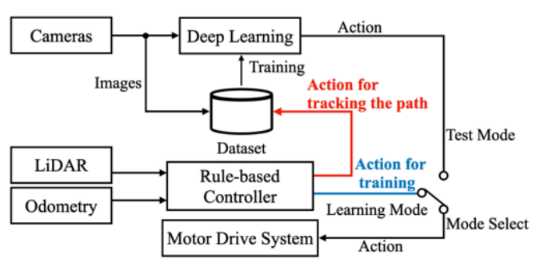
\includegraphics[width = 10cm]{./figs/okada_sys.png}
    \caption{Okada and others proposed method from \cite{okada}}
    \label{fig::okada_sys}
\end{figure}

\begin{figure}[h]
    \centering
    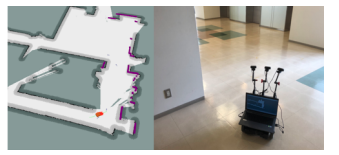
\includegraphics[width = 10cm]{./figs/okada.png}
    \caption{A robot that follows a path using vision based from \cite{okada}}
    \label{fig::okada}
\end{figure}

\newpage
上記の研究により,カメラ画像用いてロボットが学習した経路を
周回可能であることが確認されている.
次に岡田ら\cite{okada}の研究(本研究では”従来手法”と呼ぶ)をベースに,Fig. \ref{fig::bunki}のような分岐路において経路選択をする機能の追加を検討する.
% 画像のみを入力としたネットワークでは,分岐路においてネットワークが2つの方向を出力してしまい,
% 左右に車体を向ける振動が発生してしまう事象がDean A. Pomerleauら\cite{pomeru}によって確認されている.
% そこで経路を選択するために必要な情報の検討を行う.
 \vspace{4.0zh}
\begin{figure}[h]
    \centering
    \includegraphics[width = 8cm]{./figs/bunki.pdf}
    \caption{Cross road}
    \label{fig::bunki}
\end{figure}
\newpage
島田らは人が目的地までの移動に用いる道案内の情報を,
トポロジカルマップとシナリオを用いて表現する手法を提案している.
トポロジカルマップとはFig. \ref{fig::topo}に示す通路の特徴とエッジの情報をもち、
分岐路などの目印(エッジ)とそのつながり(ノード)を簡易的に表現した地図である,
シナリオは\ref{fig::sina}に示すトポロジカルマップを用いて,
「次の角まで」のような「条件」と「直進」などの「行動」の組み合わせた経路の情報である.
この研究により,「直進」「右折」などの情報で経路を選択することが可能であると示されている.
\begin{figure}[H]
    \centering
    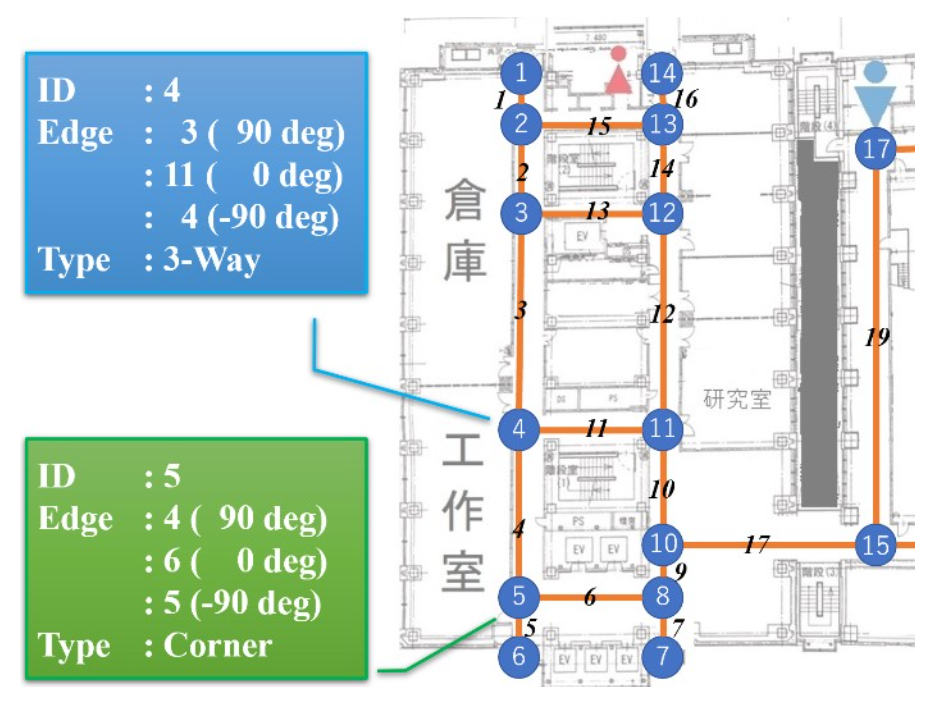
\includegraphics[width = 13cm]{./figs/topo.png}
    \caption{Topological map from\cite{simada}}
    \label{fig::topo}
\end{figure}
\begin{figure}[H]
    \centering
    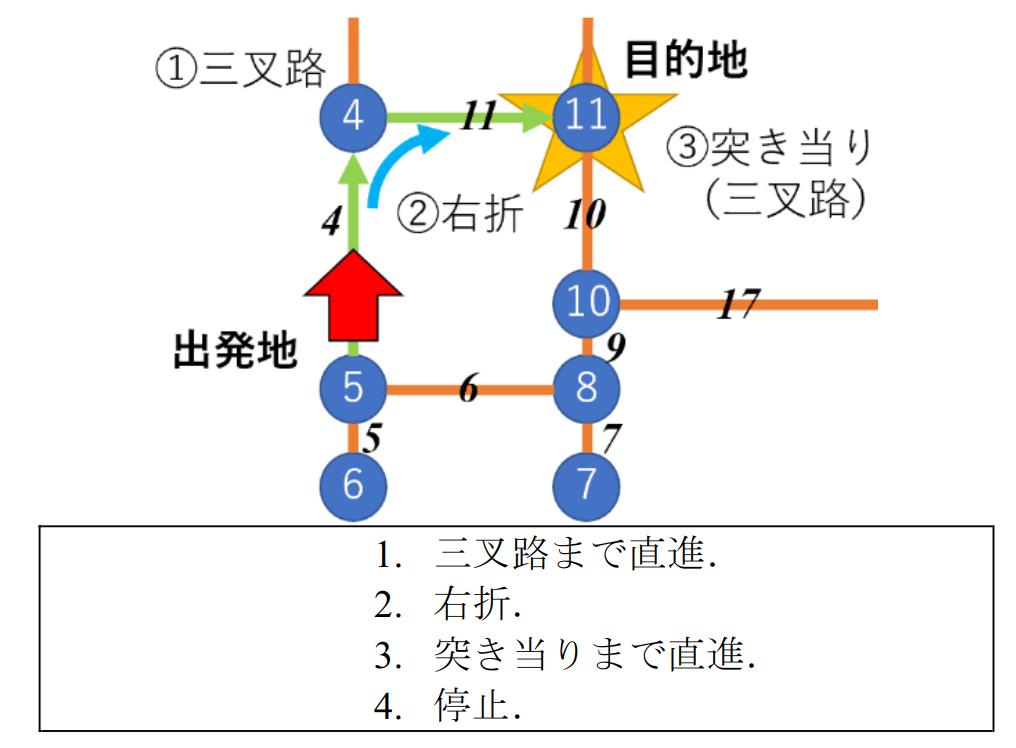
\includegraphics[width = 13cm]{./figs/sina.png}
    \caption{Scenario of the trajectory from \cite{simada}}
    \label{fig::sina}
\end{figure}

そこで,本研究では従来手法をベースに,「直進」「左折」「右折」などの目標とする進行方向の情報(本研究では"目標方向"と呼ぶ)
をデータセットと学習器へ与える.
これにより,学習器の出力を用いた走行において,目標方向により経路を選択可能とする機能の追加を提案する.
% 提案手法全体の流れをFig. \ref{fig::haikei_zentai}に示す.
% \begin{figure}[H]
%     \centering
%     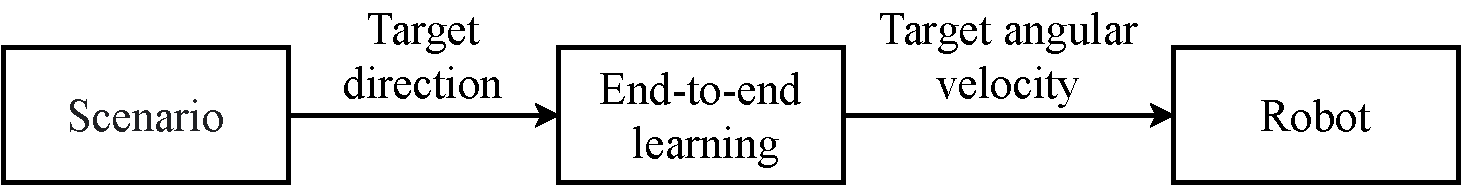
\includegraphics[width = 13cm]{./figs/haikei_zentai.pdf}
%     \caption{hai}
%     \label{fig::haikei_zentai}
% \end{figure}

\newpage
カメラ画像と他の情報を用いて,自律移動を行う研究として
Felipeら\cite{razikon}はカメラ画像と操舵角と加速度の2次元の制御信号と,continue,left,straight,rightの4つのコマンドを入力としたネットワークを
用いてFig. \ref{fig::Conditional_Imitation_Learning}で示すように実環境と都市環境のシミュレータ上で学習器がコマンドに沿った行動が可能であることを
確認している.
\begin{figure}[H]
    \centering
    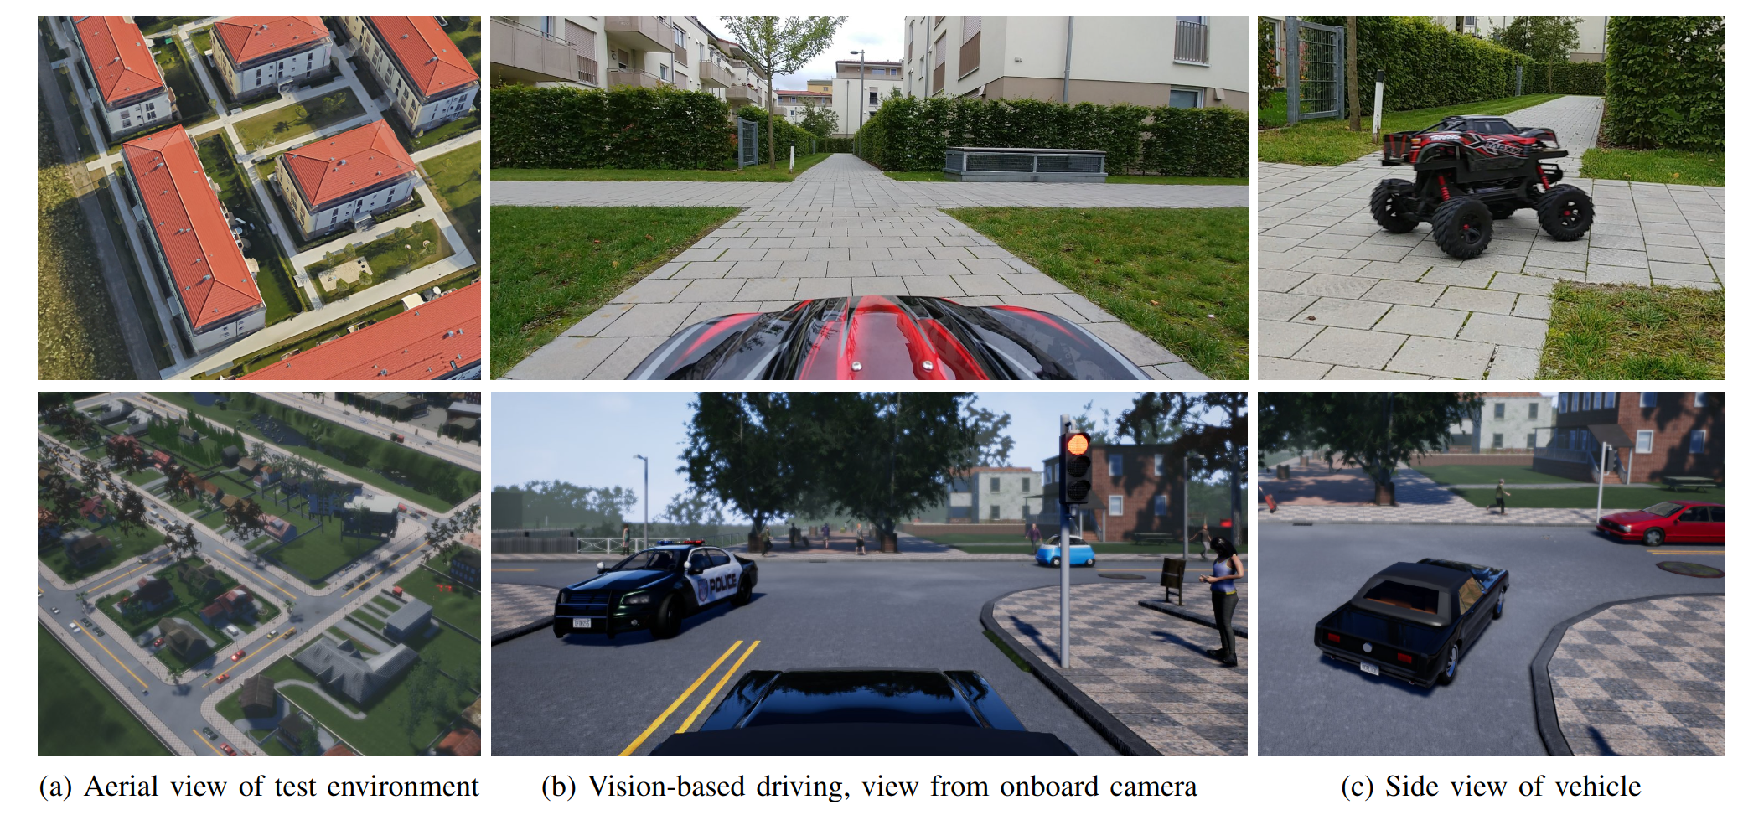
\includegraphics[width = 12cm]{./figs/End-to-end_Driving_via_Conditional_Imitation_Learning.pdf}
    \caption{End-to-end  driving  via  conditional  imitation  learning from \cite{razikon}}
    \label{fig::Conditional_Imitation_Learning}
\end{figure}

また,Seiyaら\cite{nagoya}はFig. \ref{fig::nagoyaabst}で示すように
カメラ画像と目標方向を入力,ステアリング制御信号を出力とするシステムを用いて,右および左に曲がる屋外の軌道を
追跡可能であることを確認している.

\begin{figure}[H]
    \centering
    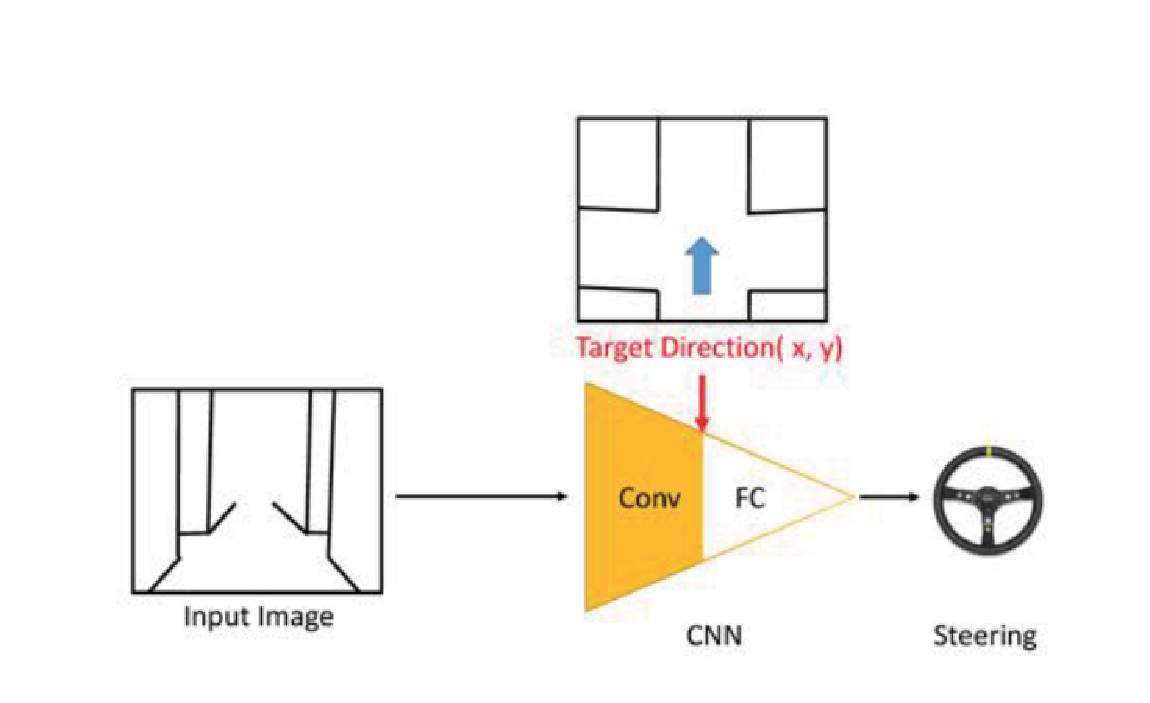
\includegraphics[width = 9cm]{./figs/End-to-End_Navigation_with_Branch_Turning_Support_using_Convolutional_Neural_Network_abst.pdf}
    \caption{Overview of Seiya and others proposed method from \cite{nagoya}}
    \label{fig::nagoyaabst}
\end{figure}


\section{目的}
本研究では,従来手法をベースに,
分岐路で「直進」と「左折」などの経路を選択可能とする機能の追加を提案する.
さらに,実験を行い,提案手法の有効性を検証することを目的とする
% Fig. \ref{fig::haikei_abs}に赤枠で示した部分を対象とする,
% \begin{figure}[H]
%     \centering
%     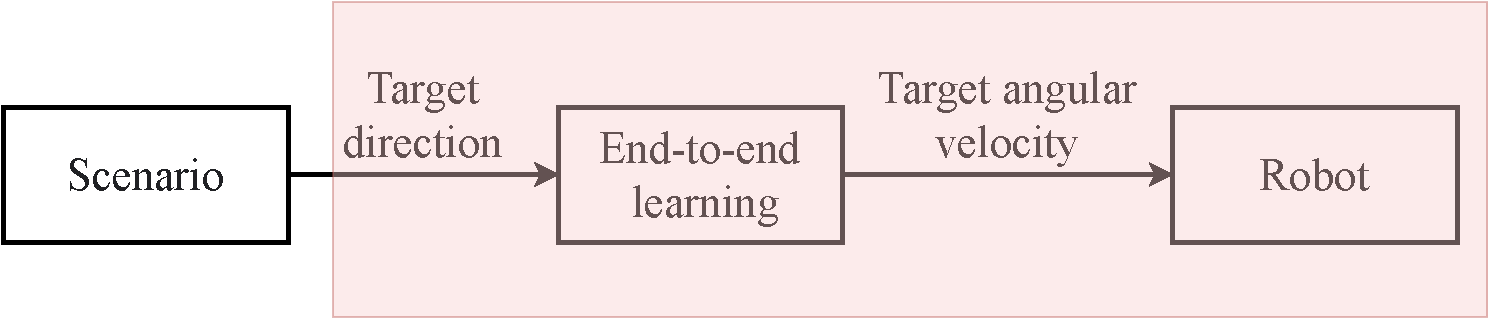
\includegraphics[width = 12cm]{./figs/haikei_abs.pdf}
%     \caption{a}
%     \label{fig::haikei_abs}
% \end{figure}

% カメラ画像と目標方向を入力とする学習器の出力を用いた走行において,
% 目標方向によって分岐路で任意のルートへ走行経路を変更することを目指す.
% カメラ画像以外に分岐路での方向指示の情報を追加し,その情報を用いてルート選択が可能であるかの
% 検証を行う.


\section{論文構成}
1章では,本研究における背景,及び目的を述べた.
2章では,本研究で用いた深層学習の要素技術とベースとする従来手法について述べる.
3章では,本研究で用いた手法と構築したシステムについて述べる.
4章では,構築したシステムを用いた実験を行う.
5章では,本研究の結論を述べる.
